\documentclass{article}
\usepackage[submission]{colm2026_conference}

% Encoding & typography
\usepackage[T1]{fontenc}
\usepackage[utf8]{inputenc}
\usepackage{microtype}

% Colors & hyperlinks
\usepackage[dvipsnames]{xcolor}
\definecolor{darkblue}{rgb}{0, 0, 0.5}
\usepackage{hyperref}
\hypersetup{colorlinks=true, citecolor=darkblue, linkcolor=darkblue, urlcolor=darkblue}
\usepackage{url}
\usepackage{lineno}

% Math & symbols
\usepackage{amsmath,amssymb,amsfonts,amsthm,mathtools,bm,dsfont}
\usepackage{nicefrac,xfrac}

% Algorithms
\usepackage{algorithm}
\usepackage{algorithmic}

% Tables & figures
\usepackage{graphicx}
\usepackage{subcaption}
\usepackage{wrapfig}
\usepackage{booktabs}
\usepackage{multirow}
\usepackage{makecell}
\usepackage{colortbl}
\usepackage{adjustbox}
\usepackage{array}
\usepackage{tabularx}
\usepackage{rotating}
\usepackage{arydshln}

% Code
\usepackage{listings}

% TikZ & icons
\usepackage{tikz}
\usetikzlibrary{arrows.meta,positioning}
\usepackage{fontawesome5}

% Lists
\usepackage{enumitem}
\setlist[itemize]{noitemsep, topsep=4pt}
\setlist[enumerate]{noitemsep, topsep=4pt}

% Caption spacing
\usepackage{caption}
\captionsetup{skip=7pt}

% Float spacing
\setlength{\textfloatsep}{10pt plus 3pt minus 3pt}
\setlength{\floatsep}{10pt plus 3pt minus 3pt}
\setlength{\intextsep}{10pt plus 3pt minus 3pt}

% Math display spacing
\setlength{\abovedisplayskip}{9pt plus 3pt minus 3pt}
\setlength{\belowdisplayskip}{9pt plus 3pt minus 3pt}
\setlength{\abovedisplayshortskip}{6pt plus 2pt minus 2pt}
\setlength{\belowdisplayshortskip}{6pt plus 2pt minus 2pt}

% Bibliography spacing
\setlength{\bibsep}{1pt plus 0.4ex}

% Listings style
\lstset{
  aboveskip=6pt, belowskip=6pt,
  basicstyle=\ttfamily\scriptsize,
  frame=single,
  numbers=none
}

\title{Trusting the Formal Judge: Certifying LLM Theorem Scorers for Code Verification in Lean~4}

% Authors must not appear in the submitted version (handled automatically by the "submission" option).
\author{Anonymous}

\begin{document}

\ifcolmsubmission
\linenumbers
\fi

\maketitle

\begin{abstract}
Formal methods provide unparalleled rigor in software verification, and with the advent of AI systems, we are beginning to see their potential realized at scale; however, evaluating the quality of the theorems and specifications these systems generate remains a critical bottleneck.
Traditional benchmarks often provide a fixed theorem statement, but agentic systems must infer and synthesize these properties on their own, demanding a scalable and reliable evaluation method.
We present an LLM-based judge designed to score the quality of generated Lean~4 theorems based on correctness, completeness, and semantic alignment with a reference implementation.
More importantly, we introduce a novel methodology to certify the judge's trustworthiness by verifying its adherence to fundamental logical properties.
We demonstrate that our judge satisfies identity (identical inputs yield maximal scores) and monotonicity (scores decrease predictably as bugs are introduced or specifications are removed), with Pearson correlations up to 0.973.
By applying this validated judge to the \textsc{VeriBench}\citep{veribench_icml25} scalable oversight benchmark, we show that agentic approaches for formal code generation significantly outperform baseline prompting, with a top score of 0.615 vs.\ 0.470.
This work provides a blueprint for creating and validating reliable automated judges, enabling robust and scalable evaluation of next-generation theorem-proving agents.
\end{abstract}

\section{Introduction}

Agentic AI systems are emerging as a powerful tool for formal code verification, capable of not just proving theorems but also generating the code and the theorems themselves. This end-to-end synthesis presents a profound evaluation challenge. In traditional auto-formalization benchmarks, models are given a precise natural language statement to formalize. However, in a more realistic, agentic setting, the system must infer and propose relevant theorems from a source program and its docstring. This autonomy makes manual evaluation intractable and requires automated, scalable solutions \citep{zhou2025graders,khattab2024dspy,cheng2024trace}.

We propose a radical approach: use LLMs themselves as judges of specification quality. But can you really trust such a judge? An unreliable judge can produce misleading results, rewarding stylistic mimicry over semantic correctness and hindering genuine progress. Without a principled validation method, LLM-based evaluation remains ad hoc and its results questionable \citep{Kocmi2024HumanVsLLM,Li2024TrustLLMJudgments}.

In this paper, we present evidence indicating that it is possible to trust an LLM judge. We introduce an LLM judge for scoring the quality of synthesized theorems in Lean~4 and, crucially, present a methodology for validating its trustworthiness. We demonstrate that an LLM judge, when properly validated, can serve as a reliable proxy for human evaluation, enabling the scalable assessment of complex, agentic systems.

Our \textbf{contributions} are:
\begin{enumerate}
    \item \textbf{An LLM Judge for Theorem Quality:} We design an LLM judge that scores generated Lean~4 artifacts on a 0--10 scale based on correctness, completeness, and semantic alignment.
    \item \textbf{A Trustworthiness Validation Methodology:} We propose and execute a set of property checks to certify the judge's reliability and trustworthiness, verifying its adherence to logical properties like identity and monotonicity under controlled perturbations.
    \item \textbf{Empirical Demonstration of the Judge on \textsc{VeriBench}:} We apply our validated judge to evaluate multiple agentic frameworks, providing evidence that feedback-driven methods significantly outperform non-agentic baselines in theorem-synthesis quality.
\end{enumerate}

\section{Related Work}
\paragraph{LLM-as-a-Judge.}
LLMs are increasingly used as \emph{automated evaluators} across open-ended tasks, often reaching strong agreement with human ratings---e.g., GPT-4 judges achieving $>$80\% agreement with human preference labels in dialogue \citep{Zheng2023MTBench}. However, large-scale audits caution that reliability varies by task and setup, and stress the need for explicit validation before replacing human judgment \citep{Kocmi2024HumanVsLLM,Li2024TrustLLMJudgments}. Common biases include position and verbosity effects and sensitivity to prompt phrasing \citep{Zheng2023MTBench,Li2024TrustLLMJudgments}.

\paragraph{Improving judge reliability.}
To mitigate biases and instability, multi-agent debate frameworks such as \emph{ChatEval} emulate panel-style review to yield more robust consensus scores \citep{Chan2024ChatEval}. Structured prompting like \emph{G-Eval} elicits rubric-driven, stepwise reasoning prior to scoring, improving agreement with human criteria on NLG tasks \citep{Liu2023GEval}. Reliability can also be quantified via repeated scorings and internal consistency measures (e.g., Cronbach's $\alpha$) to detect prompt/run sensitivity \citep{Li2024TrustLLMJudgments}.

\paragraph{Code and formal-spec evaluation.}
For programming, single-pass metrics like pass@k can be brittle or unavailable; early LLM-judge approaches such as \emph{ICE-Score} highlighted difficulty distinguishing partial vs.\ full correctness from a one-shot review \citep{Zhuo2024ICEScore}. \emph{CodeJudge} operationalizes a two-stage ``analyze-then-summarize'' procedure with a taxonomy of code faults, significantly improving correlation with functional ground truth \citep{TongZhang2024CodeJudge}. In formal verification/autoformalization, prior work typically provides fixed target theorems, reducing evaluation to proof success. In contrast, agentic systems must propose specifications, necessitating \emph{semantic} judges. We adopt a certification protocol (akin to metamorphic testing) and verify that our LLM judge obeys \emph{identity/consistency} and \emph{monotonicity} with respect to injected bugs and specification omissions, directly answering recent calls for validated, trustworthy LLM evaluators in safety-critical domains \citep{Kocmi2024HumanVsLLM,Li2024TrustLLMJudgments}.

\paragraph{Overview of \textsc{VeriBench}.}
Concretely, \textsc{VeriBench} consists of 857 theorems divided into five subsets:
\begin{enumerate}
    \item \textbf{HumanEval} -- 387 theorems derived from 56 standard programming puzzles from \citet{chen2021evaluating};
    \item \textbf{EasySet} -- 278 theorems extracted from 41 introductory logic and programming tasks;
    \item \textbf{CSSet} -- 68 theorems drawn from 10 classical data-structure and algorithm problems;
    \item \textbf{SecuritySet} -- 112 theorems taken from 28 examples of buffer overflows, privilege escalation, and race-condition labs based on real code;
    \item \textbf{RealCodeSet} -- 12 theorems extracted from 5 Python standard library programs, used to test model performance on production-grade code.
\end{enumerate}
This design covers a spectrum of tasks, from simple correctness theorems to more complex invariants, algorithmic properties, and real-world code verification. See the ICML AI4Math workshop poster for \textsc{VeriBench} for additional context \citep{veribench_icml25}.

\section{Methodology: A Certification Protocol for LLM Judges}

\paragraph{Why is an LLM judge needed for theorem-quality scoring?}
Evaluating AI-generated theorems/specifications requires a method to assess their quality, as proof assistants can verify a proof's correctness but not whether the agent proved the correct theorem.
This is challenging because proving the logical equivalence of two arbitrary theorem statements is generally undecidable, and an agent may generate theorems that are semantically valid but syntactically different or incomparable with the gold reference specification/theorem (e.g., by splitting a theorem into different parts).

Our goal is to certify the trustworthiness of an LLM judge for the task of formal specification/theorem generation.
This is akin to scoring the quality of a conjecture.
We operationalize this by requiring the judge to compare a candidate Lean~4 artifact (implementation, tests, theorems) against its gold-standard Lean~4 reference.
We provide the full set of Lean~4 artifacts because theorems might not make sense in isolation.
The judge returns a discrete score $s\in\{0,1,\dots,10\}$ for correctness, completeness, and semantic alignment, which we later normalize to $[0,1]$.
We use this score as a metric signal for evaluating the specifications generated by the agents.

To be considered trustworthy, the judge must satisfy the following falsifiable properties.
These are necessary conditions for trust: they certify that the judge reacts logically to structured perturbations.

\paragraph{P1 --- Identity \& Consistency.}
The judge must be idempotent at the maximum score when comparing an artifact to itself.
For any reference $X$, it must hold that $s(X,X)=1$.

\paragraph{P2 --- Monotonicity to Bugs.}
The judge's score must decrease as semantic bugs are cumulatively introduced. Let $B_1$ and $B_2$ be sets of bugs such that $B_1 \subset B_2$. For candidates $C_{B_1}$ and $C_{B_2}$ containing precisely these bug sets, the expected scores must satisfy $\mathbb{E}[s(C_{B_1})] > \mathbb{E}[s(C_{B_2})]$.

\paragraph{P3 --- Monotonicity to Missing Specs.}
The judge's score must decrease as specification elements are removed.
Let $S_1$ and $S_2$ be sets of specifications (theorems and tests) such that $S_2 \subset S_1$.
For candidates $C_{S_1}$ and $C_{S_2}$ containing precisely these specification sets, the expected scores must satisfy $\mathbb{E}[s(C_{S_1})] > \mathbb{E}[s(C_{S_2})]$.

\paragraph{Certification Protocol.}
We implement three scripted perturbation families on the \emph{candidate} while holding the \emph{gold} fixed:
(i) \emph{Identity} (P1), pairing each gold file with itself (and a semantically identical reflow) to test idempotence robustness;
(ii) a \emph{Bug Ladder} (P2), applying $k\!\in\!\{0,\ldots,K\}$ semantics-changing transformations (e.g., broken identities, violated commutativity, incorrect base cases); and
(iii) \emph{Specification Ablation} (P3), removing $m\!\in\!\{0,\ldots,M\}$ theorems or tests.
We then verify monotonicity by computing rank correlations (Kendall's $\tau$, Spearman's $\rho$) between $(k,m)$ and judged scores, and by reporting pairwise ordering accuracy (AUC) that ``worse'' artifacts receive lower scores \citep{TongZhang2024CodeJudge,Zhuo2024ICEScore}.

\textbf{Establishing trust in the LLM judge.} To ensure trustworthiness of the LLM judge in evaluating agentic autoformalization, we systematically validate key properties the judge must satisfy in Figure~\ref{fig:judge_sanity_checks}: (1) scores decrease consistently as more theorems and tests are omitted, (2) scores similarly degrade when more implementation bugs are introduced, and (3) identical file pairs always yield maximal scores.
Empirical results confirm these properties strongly hold (Pearson correlations up to $-0.973$), thus validating that our Claude~3.5-based LLM judge provides a reliable and semantically meaningful measure for correctness, completeness, and alignment of autonomously inferred theorems across \textsc{VeriBench} subsets (Table~\ref{tab:theorem_quality_table_split}) \citep{Li2024TrustLLMJudgments,Kocmi2024HumanVsLLM}.

\begin{figure*}[t]
  \centering
  \begin{subfigure}[t]{0.315\textwidth}
    \centering
    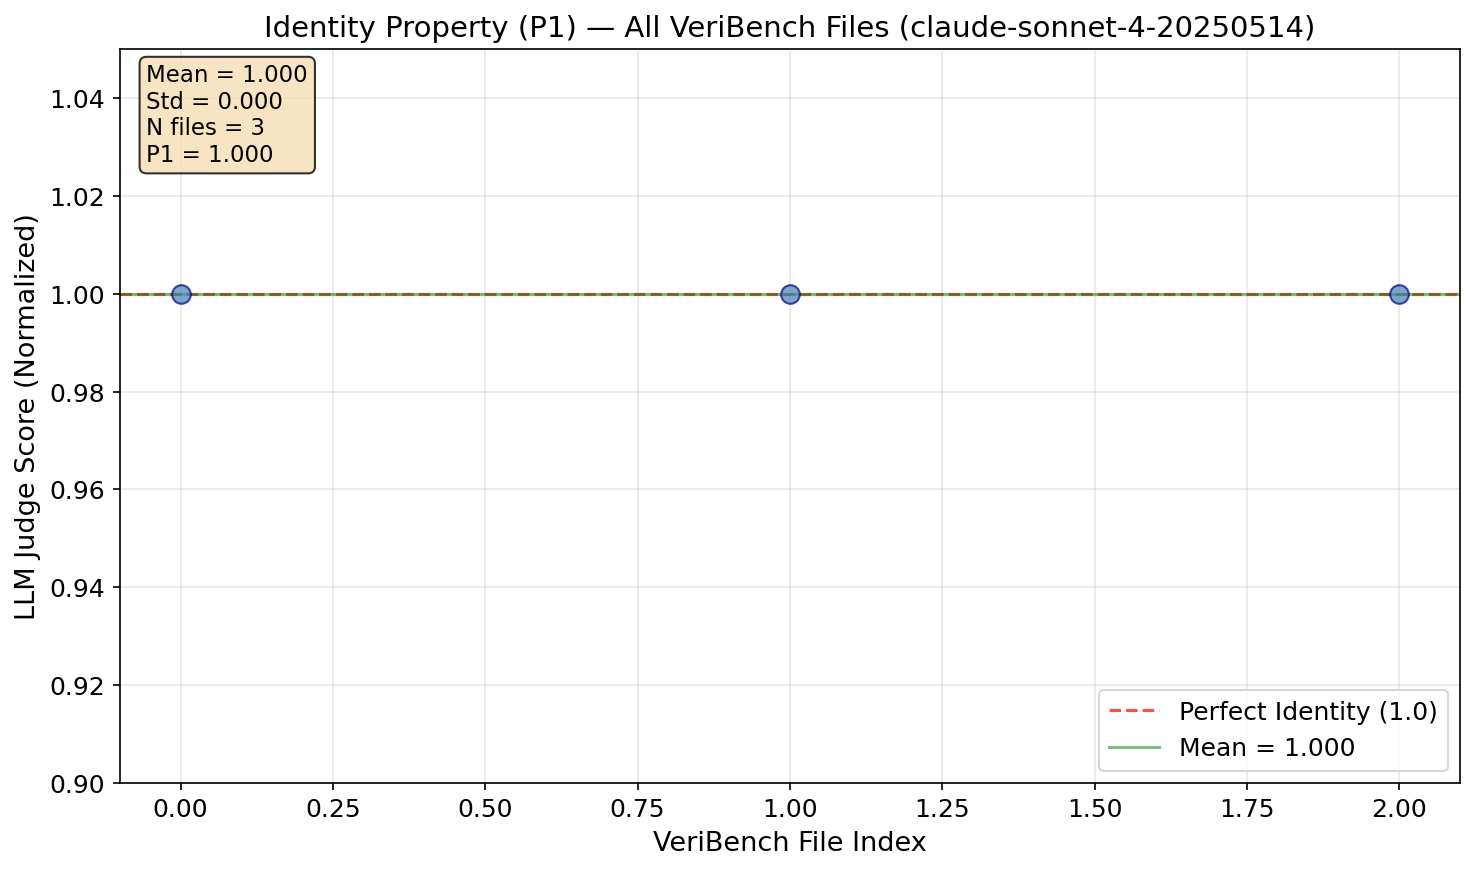
\includegraphics[width=\linewidth]{figures/identity_property.png}
    \caption{Identity (Reflexivity)}
    \label{fig:judge_identity}
  \end{subfigure}\hfill
  \begin{subfigure}[t]{0.315\textwidth}
    \centering
    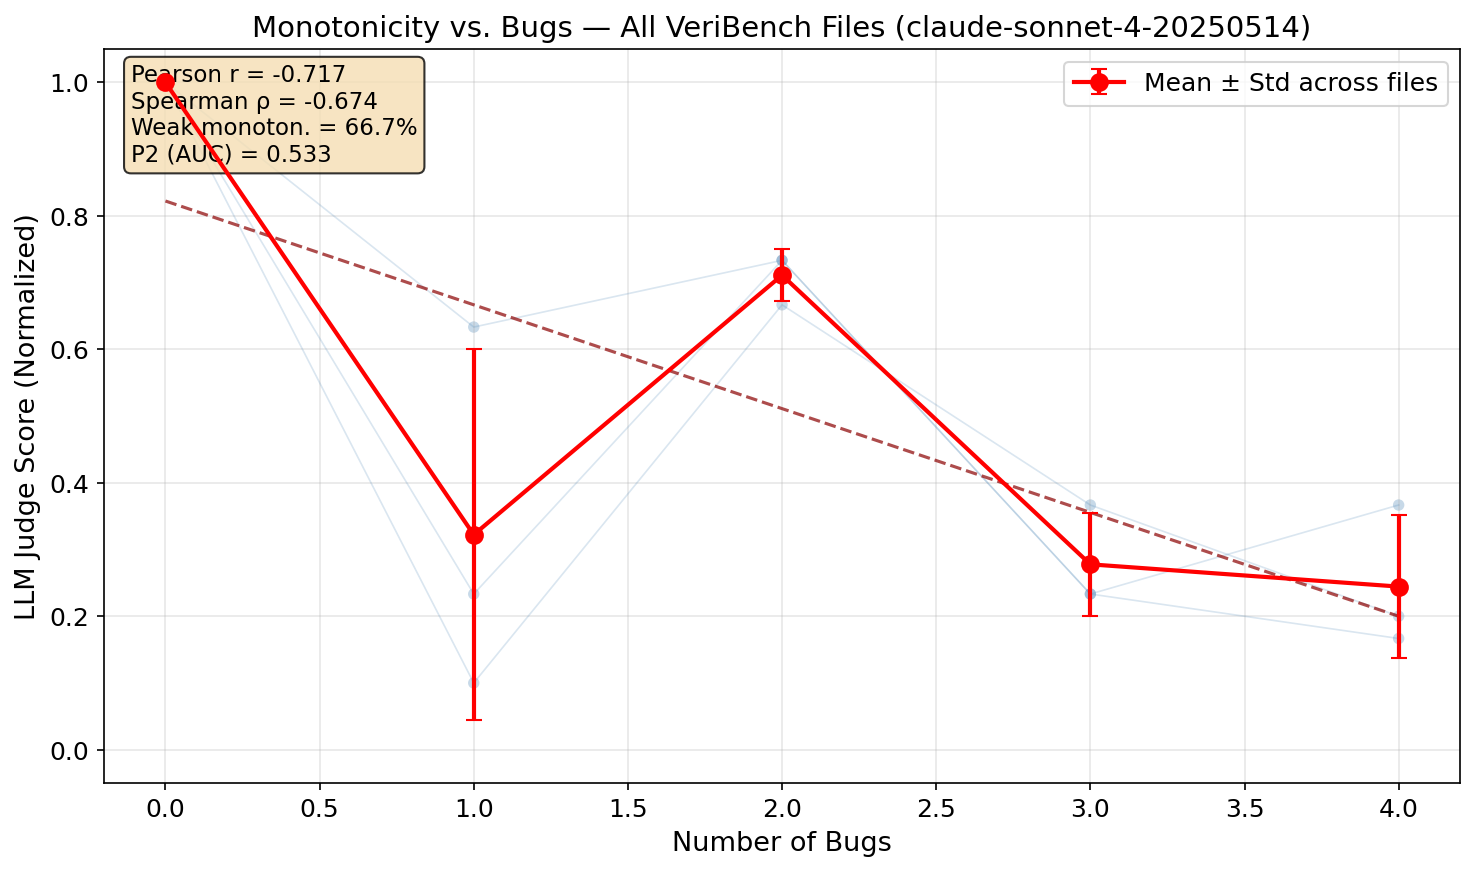
\includegraphics[width=\linewidth]{figures/monotonicity_bugs.png}
    \caption{Monotonicity vs.\ Bugs}
    \label{fig:judge_mono_bugs}
  \end{subfigure}\hfill
  \begin{subfigure}[t]{0.315\textwidth}
    \centering
    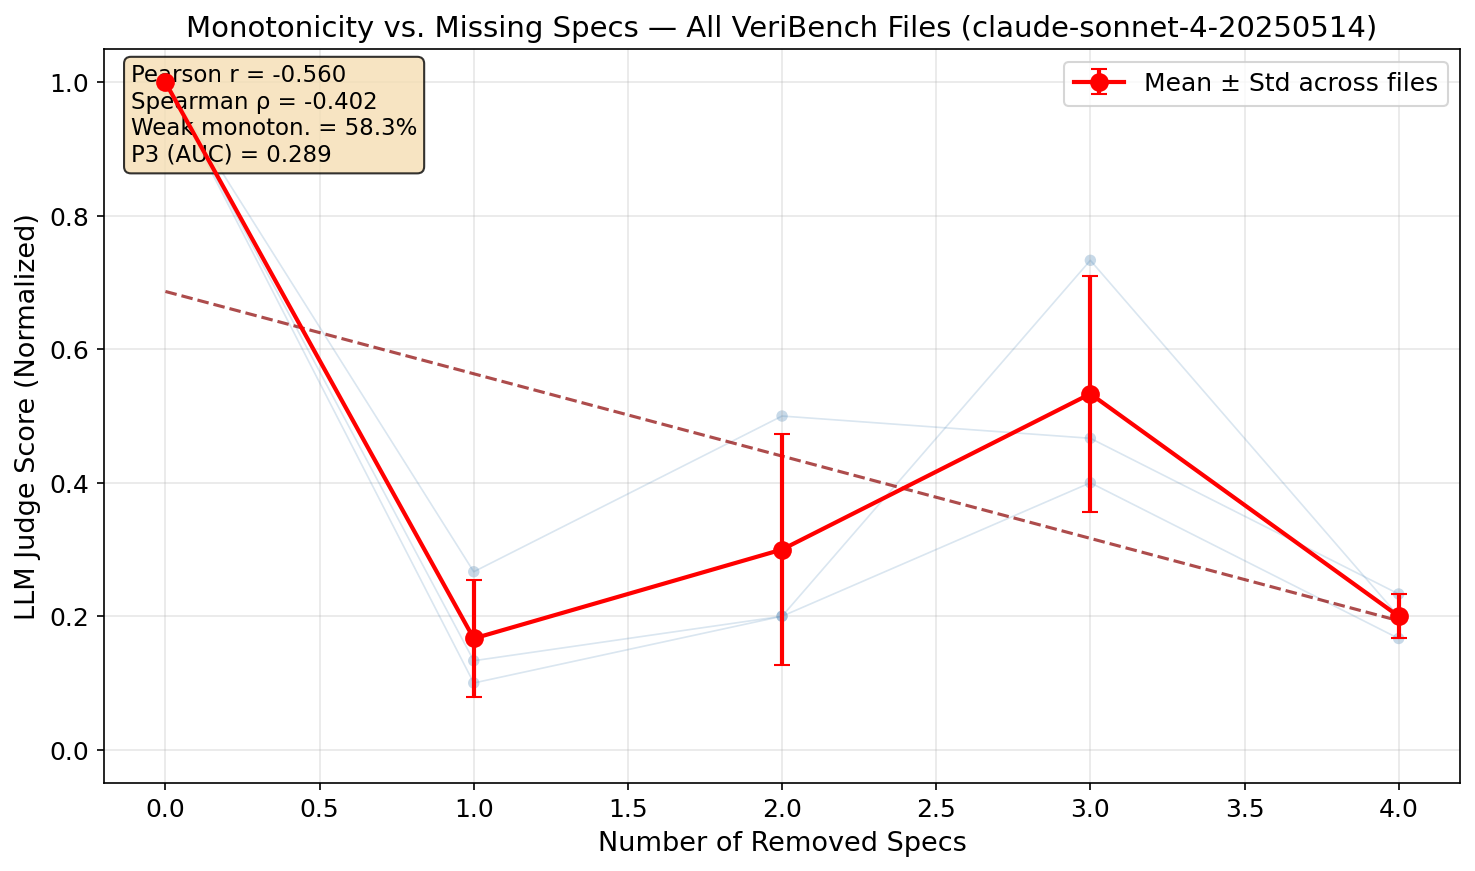
\includegraphics[width=\linewidth]{figures/monotonicity_missing_specs.png}
    \caption{Monotonicity vs.\ Missing Specs}
    \label{fig:judge_mono_specs}
  \end{subfigure}
  \vspace{-2mm}
\caption{\textbf{LLM Judge Trustworthiness Sanity Checks.}
The judge demonstrates reliability against our certification protocol.
\textbf{(a) Identity:} When comparing a gold-standard file to itself, the judge consistently returns the maximum normalized score of 1.0 ($R^2=1.000$).
\textbf{(b) Monotonicity vs.\ Bugs:} The judge's score shows a strong negative correlation with the number of injected bugs (Pearson $r = -0.973$, Spearman $\rho = -0.985$).
\textbf{(c) Monotonicity vs.\ Missing Specs:} Similarly, the score decreases predictably as specifications are removed (Pearson $r = -0.979$, Spearman $\rho = -0.985$).}
  \label{fig:judge_sanity_checks}
  \vspace{-3mm}
\end{figure*}

\section{Results: Evaluating Agentic Theorem Generation with a Certified Judge}
Table~\ref{tab:theorem_quality_table_split} presents the normalized average scores across different splits of \textsc{VeriBench}: Easy Set (Easy), CS Set (CS), Real Python Code (Real), HumanEval Set (HE), and Security Set (Sec).
As expected, the baseline prompting approach achieves the lowest overall normalized score (0.470), reflecting its limited capability in autonomously identifying comprehensive theorem properties.
It also gives us further confidence in our judge.
Conversely, agentic methods leveraging iterative self-debugging and self-improvement demonstrate significant enhancements.
Specifically, the DSPy ReAct agent, which incorporates feedback-driven self-debugging, achieves the highest overall average score of 0.615.
The Trace++ agent, employing both self-debugging and self-improvement mechanisms, also shows notable improvement, attaining an average score of 0.588.
These results underscore the effectiveness of agentic, feedback-driven approaches in enhancing theorem-generation quality compared to non-agentic baselines \citep{khattab2024dspy,cheng2024trace,chen2021evaluating}.

\begin{table}[H]
\renewcommand{\arraystretch}{1.30}
\centering
\begin{tabular}{@{}llccccc c@{}}
\toprule
& & \multicolumn{5}{c}{\textbf{Split}} & \\
\cmidrule(lr){3-7}
\textbf{Agent} & \textbf{Eval} & \textbf{Easy} & \textbf{CS} & \textbf{Real} & \textbf{HE} & \textbf{Sec} & \textbf{Avg} \\
\midrule
\multirow{1}{*}{\makecell[l]{Baseline Prompting}}
& Normalized & 0.580 & 0.690 & 0.472 & 0.410 & 0.347 & \makecell{\textbf{0.470}} \\
\addlinespace[2pt]
\hdashline[0.5pt/4pt]
\addlinespace[2pt]
\multirow{1}{*}{\makecell[l]{\textsc{DSPy ReAct}}}
& Normalized & 0.659 & 0.754 & 0.580 & 0.650 & 0.454 & \makecell{\textbf{0.615}} \\
\addlinespace[2pt]
\hdashline[0.5pt/4pt]
\addlinespace[2pt]
\multirow{1}{*}{\makecell[l]{\textsc{Trace+} (Self-Debug)}}
& Normalized & 0.342 & 0.680 & 0.592 & 0.573 & 0.411 & \makecell{\textbf{0.477}} \\
\addlinespace[2pt]
\hdashline[0.5pt/4pt]
\addlinespace[2pt]
\multirow{1}{*}{\makecell[l]{\textsc{Trace++} (Self-Improve)}}
& Normalized & 0.620 & 0.756 & 0.504 & 0.645 & 0.432 & \makecell{\textbf{0.588}} \\
\bottomrule
\end{tabular}
\caption{\textbf{Theorem Quality Scores.} Average normalized scores in \textsc{VeriBench} split: Easy Set (Easy), CS Set (CS), Real Python Code (Real), HumanEval Set (HE), Security Set (Sec).
All rows use Claude~3.7 as the agent model and as the LLM judge.
Trace+ denotes the trace self-debug agent and Trace++ the self-debug and self-improve agent.
The DSPy ReAct agent only performs self-debug.
The LLM judge issues 5 scoring calls per file pair and returns an integer rubric score in $\{0,1,\dots,10\}$.
Normalized scores are computed by dividing by the maximum score (10) and averaging across all examples.
The Avg Norm Score shows the overall average over the entire benchmark.}
\label{tab:theorem_quality_table_split}
\end{table}

\section{Discussion, Limitations, and Future Work}
We study an LLM judge that \emph{compares each candidate artifact against its task's gold reference} for Lean~4 code verification and a framework to increase confidence in it.
The judge satisfies two falsifiable properties: (i) \textbf{identity}---gold vs.\ gold yields maximal, repeatable scores; and (ii) \textbf{monotonicity}---scores decrease predictably when we inject semantic bugs or ablate specification elements.
In experiments, certified judging produces informative method rankings and tracks engineering signals (Pass@$k$, unit-test accuracy); Easy and HumanEval show the strongest agreement, while Security and RealCode remain hardest \citep{chen2021evaluating}.

\textbf{Limitations.} The judge is a \emph{proxy}: scores are prompt/rubric-sensitive and do not constitute kernel-level proof checking; they certify agreement with a rigorous yet necessarily incomplete gold specification since no complete mechanical checks of specification equivalence exist~\citep{rice1953}.
Our certification relies on a finite perturbation suite, so untested failure modes may persist. Specifications that are exotic to this dataset may be correct but receive incorrect scores.
We also did \emph{not} collect human expert ratings, leaving the judge--human correlation unmeasured.
Future work will add human validity studies (correlations and reliability), strengthen semantic equivalence handling (candidate $\Rightarrow$ gold postcondition checks), expand robustness and adversarial tests, and introduce uncertainty reporting and standardized ``judge cards'' for reproducible, certified use \citep{zhou2025graders}.

\bibliography{refs}
\bibliographystyle{colm2026_conference}

\appendix

\section{Related Work (Cont.)}

\paragraph{Autoformalization.} Complementing this line of work, \citet{wang2024theoremLlama} present \textsc{TheoremLlama}, a framework aimed at enhancing LLM translation into Lean 4. Drawing on over 100K proof examples from the Mathlib4 library, TheoremLlama employs a novel natural-language-to-formal-language (NL-FL) bootstrapping strategy and iterative proof synthesis. This enables the reuse of verified examples as templates for future translations. The framework achieves 36.48\% and 33.61\% accuracy on the MiniF2F-Valid and MiniF2F-Test benchmarks, respectively---surpassing GPT-4 by more than ten percentage points on both.

\textbf{Techniques for Code Verification.}
\textsc{ImProver}~\citep{ahuja2024improver} introduces a Lean-aware Chain-of-States prompting loop that integrates retrieval, best-of-$n$ sampling, and iterative correction to rewrite formal proofs with improved properties. By optimizing for metrics such as brevity and readability, ImProver reduces the number of tactics by half, doubles proof readability, and boosts theorem prover acceptance rates by over 80\%.
In addition, \textsc{Clover}~\citep{sun2024clover} implements a closed-loop pipeline in which an LLM first generates code, docstrings, and formal annotations, then uses reconstruction-based prompting to enforce consistency across these outputs, and finally applies SMT-based verification to validate correctness. Evaluated on the CloverBench suite of Dafny programs, Clover accepts 87\% of correct solutions, rejects 100\% of flawed ones, and even uncovers bugs in human-written code---demonstrating the power of hybrid generation-verification pipelines.
In a complementary direction, \citet{zhou2025graders} improve general-purpose LLM-based graders by augmenting them with ``privileged'' information such as gold-standard solutions, grading rubrics, and detailed annotations. When necessary, the system provides targeted hints back to candidate models. This approach achieves grading performance on par with or exceeding that of specialized systems---and even expert humans---on difficult programming benchmarks.

\textbf{Agentic Frameworks and Tools for Code Verification.}
\textsc{Trace}~\citep{cheng2024trace} proposes \emph{generative optimization}, tuning entire computational workflows---including code, prompts, tool calls, and error signals---by treating execution traces as gradients in the OPTO framework. With a PyTorch-like API and the LLM-based optimizer OptoPrime, it supports diverse tasks such as prompt tuning, debugging, and robot control, rivaling specialized optimizers.
Building on modular composition, \textsc{DSPy}~\citep{khattab2024dspy} treats LLM calls as declarative modules in a computational graph. Users define concise input--output signatures, and DSPy's compiler automatically bootstraps or fine-tunes pipelines using built-in ``teleprompters.'' This enables a few-line programs to outperform expert-crafted prompts in math, QA, and agent workflows.
Extending agentic capabilities to formal reasoning, \textsc{Pantograph}~\citep{aniva2025pantograph} offers a programmatic interface to Lean 4 with support for advanced proof search. It exposes internal proof states and tactics for integration with learning agents, replacing human-facing interfaces with API-level control.

\subsection{Related Work: Scalable Oversight}

\paragraph{Scalable Oversight with LLM Judges}
Researchers have proposed multi-agent oversight frameworks such as debate and consultancy, where weaker LLMs act as judges supervising stronger agents \citep{kenton2024oversight,Chan2024ChatEval}.
Debate, in which two models argue opposing sides before a judge, consistently improves truth-tracking compared to single-pass QA. \citet{kenton2024oversight} demonstrate that debate reduces the likelihood of judges being misled in math and code tasks, highlighting it as a scalable oversight mechanism.

\paragraph{Self-Improving Critics.}
In the absence of stronger supervisors, models can bootstrap judgment skill through self-critique.
The Self-Evolving Critic (SCRIT) framework trains LLMs to generate critiques of flawed outputs, validate corrections, and iteratively refine their ability to spot errors. \citet{zheng2024scrit} report improvements of over 10\% on critique benchmarks, showing that self-critique fosters scalable, autonomous oversight.

\paragraph{Certifying Judges.}
Naïve LLM judges are often inconsistent, rewarding stylistic cues over correctness \citep{Kocmi2024HumanVsLLM,Li2024TrustLLMJudgments}.

\paragraph{Validity-Centered Evaluation.}
Certifying judges requires not only behavioral properties but also principled validity evidence. \citet{salaudeen2025measurement} introduce a framework that distinguishes between measurement, claims, and evidence, grounded in psychometrics. They emphasize construct, content, and criterion validity, and systematically enumerate threats to validity. This framework provides a blueprint for reporting and interpreting judge certification results, complementing identity/monotonicity checks with broader validity cards.

\paragraph{Robust Evaluation without Ground Truth.}
Standard judge queries can be brittle in the absence of ground truth, particularly under adversarial manipulation \citep{Zhuo2024ICEScore,TongZhang2024CodeJudge}. \citet{robertson2025stepbystep} model the overseer as an agent and propose using information-theoretic, incentive-compatible queries instead of direct ratings. They introduce bounded $f$-divergence measures such as TVD-MI, which exhibit polynomial robustness to adversarial strategies, unlike unbounded KL-based criteria. This work highlights a pathway toward robust, certifiable judges when explicit ground truth is unavailable.

\paragraph{Formal Methods as Oversight.}
Proof assistants provide binary, kernel-level guarantees. \citet{zhou2024donttrustverify} autoformalize math solutions into Isabelle/HOL and show that filtering via proof checking outperforms majority voting by 12\% on GSM8K. \citet{liu2025safe} extend this approach with SAFE, which verifies every intermediate step in Lean 4 and introduces the FormalStep benchmark, reducing hallucinations and enabling fine-grained oversight.

\paragraph{Agentic Iterative Pipelines.}
\citet{ospanov2023apollo} integrate Lean feedback into recursive repair cycles, boosting general-purpose LLM proof success from 3--7\% to over 40\% on miniF2F, and achieving 75\% with fewer than 1000 samples. \citet{miranda2025veribench} extend this paradigm to program verification, showing that self-debugging agents quadruple success compared to one-shot prompting.
Incorporating an LLM judge improved completeness on security tasks but required calibration to avoid regressions on simpler cases.

\paragraph{Benchmarks for Judge Reliability.}
Benchmarks such as VeriBench and FormalStep quantify judge reliability across compilation, proof success, and specification quality.
\citet{miranda2025veribench} report normalized specification scores of 0.470 for one-shot prompting versus 0.615 for self-debugging agents.
Outside formal mathematics, MT-Bench and G-Eval provide complementary judge-evaluation settings using pairwise preferences and rubric-guided scoring, underscoring the need for calibration and validity reporting \citep{Zheng2023MTBench,Liu2023GEval}.
Together with validity frameworks and robust information-theoretic scoring, these benchmarks advance the agenda of certifying LLM judges for formal verification.

\paragraph{Evaluating Autoformalization with Reference-Free Judges.}
In a complementary line of work, \citet{zhang2025goldstandardsepistemicensemble} propose an ensemble of LLM judges for the autoformalization task, using a fine-grained taxonomy to score formalizations without a gold-standard reference.
The primary strength of this approach is its reference-free nature, offering a scalable evaluation pathway when gold standards are unavailable or prohibitively expensive to create.
However, the work's motivation for abandoning gold-standard comparison is based on limited evidence: a small, non-random sample of ``potentially incorrect'' formalizations pre-selected by an LLM, whose own reliability is uncertified.
Furthermore, the framework validates its judge by correlating with human preference scores---a subjective proxy---rather than the more objective, machine-checkable goal of logical equivalence to a known-correct specification.
Critically, even if minor errors exist in gold-standard datasets, recent work has shown that such noise rarely alters the relative ranking of models, as errors are typically correlated across systems \citep{salaudeen2024imagenot}.
This suggests that a small number of flawed examples does not invalidate the utility of an entire benchmark for comparative evaluation.
Our work, in contrast, proceeds from the basis that gold standards are sufficiently reliable for ranking and focuses on certifying a judge's logical consistency against them---which is the desirable gold metric to be using.

\subsection{HCI for Solving Scalable Oversight}

\paragraph{From more evaluation to \emph{human-centered} oversight.}
HCI reframes scalable oversight as a \emph{calibration} problem: design interactions that let people verify, steer, and place \emph{appropriate} trust in LLM outputs rather than maximizing raw trust \citep{bach2022trusthci}. Interface choices (e.g., citations, explanations, confidence cues) can substantially shift user trust---sometimes in misleading ways---so the goal is to expose process and embed lightweight verification instead of presenting one-shot answers \citep{ding2025citations}. User studies in AI pair-programming similarly surface needs to communicate model performance, provide control over output style/constraints, and expose uncertainty to avoid over-reliance \citep{wang2024trustcode}.

\paragraph{Hybrid human$\leftrightarrow$AI evaluation.}
HCI work operationalizes scalable evaluation by combining expert/lay judgments with automated judges. Humans annotate failures or verify slices of output; systems then train or condition LLM-based ``reference evaluators'' on those signals to scale up assessment while staying anchored to what users value (accuracy, safety, usefulness). This human-in-the-loop pattern complements LLM-as-judge approaches---whose reliability varies by task and setup \citep{Kocmi2024HumanVsLLM,Li2024TrustLLMJudgments}---and is especially relevant when pass@k or single-shot metrics are brittle.

\paragraph{Interfaces that \emph{operationalize} oversight.}
HCI systems instantiate oversight as interaction loops that make correctness checkable \emph{during} generation: (i) \emph{test-driven code generation} (TiCoder) elicits yes/no judgments about candidate unit tests before showing code; a few interactions reduced cognitive effort and lifted pass@1 by $\sim$45.7\% on coding benchmarks \citep{naik2024ticoder}; (ii) \emph{explain$\rightarrow$correct loops} (IntelliExplain) pair each snippet with a natural-language rationale that users can critique, improving novice task success by $\sim$11--25\% \citep{yan2024intelliexplain}; (iii) \emph{pair debugging} (HypoCompass) has humans hypothesize faults while the LLM attempts fixes, yielding $\sim$12\% learning gains \citep{ma2024hypocompass}; (iv) \emph{multi-step pipelines} (PromptChainer) expose intermediate steps (e.g., tests $\rightarrow$ verification $\rightarrow$ proof attempt), enabling user intervention where failures arise \citep{wu2022promptchainer}; and (v) \emph{source-grounded verification} (SymGen) highlights claim-level spans backed by exact sources and leaves unsupported text unhighlighted, speeding verification by $\sim$20\% and raising user confidence \citep{shen2024symgen}. Collectively, these patterns shift trust from fluency to \emph{verifiable progress}.

\paragraph{Applying HCI patterns to formal specs/theorems.}
Formal kernels (Lean/Isabelle) already deliver binary checks; HCI contributes the \emph{workflow glue} that helps users evaluate \emph{which} theorem/spec to prove and whether it is complete. Two actionable patterns: (1) \emph{counterfactual spec probes}---UI toggles that remove a postcondition or inject a known bug and display the impact on tests/judge score---help detect missing clauses or overfitting; and (2) \emph{stepwise proof oversight}---surfacing intermediate goals and marking unverified suggestions---keeps the human in control of proof search. In our setting, these patterns interface naturally with a graded, semantics-sensitive evaluator.

\subsection{Vericode}
\citet{bursuc2025benchmarkvericodingformallyverified} presumes well-formed formal specifications and evaluates end-to-end verification under those specs (in Dafny, Verus/Rust, or Lean) reporting verified pass rates.
In practice, impactful problems often lack both complete specifications and ground-truth answers.
Our \textsc{VeriBench} program targets this gap by challenging the \emph{generation} of specifications (from code, tests and documentation) and then \emph{certifying} their quality prior to proof search using a Lean-aware LLM judge that we validate via falsifiable principles/properties (Identity and Monotonicity), addressing known pitfalls of LLM-as-a-judge such as bias and prompt sensitivity \citep{Zheng2023MTBench,Kocmi2024HumanVsLLM,Li2024TrustLLMJudgments}.
However, our framework has only been tested with a judge with gold references files with specifications but we will explore metrics/methods that don't require this like TVD-MI in \citep{robertson2025stepbystep}.

Beyond spec-first settings, the Unsolved Questions (UQ) paradigm evaluates models on difficult, real-world problems that have neither ground-truth answers nor formal specifications; instead, it relies on validator pipelines and community verification to track progress without oracles \cite{nie2025uqassessinglanguagemodels,uq2025}.
Taken together, these lines of work shift evaluation from ``solve what is already specified'' to ``specify, certify, then solve'':
vericoding provides end-to-end rigor under given specs, \textsc{VeriBench} adds specification synthesis with a certified semantic judge, and UQ extends evaluation to specless, answerless settings that require validator-assisted screening.
Our contribution is a certified, semantics-sensitive judge that enables scalable oversight when the specification must be proposed rather than merely proved.
Because specification generation often lacks a unique ground truth, we will extend our oracle-free certification protocol with UQ-style validators, adding cycle-consistency tests (spec to code/docs) alongside our bug and ablation ladders, and enabling abstention when validators disagree to prioritize precision over coverage.

\section{Discussion (Cont.)}
\textbf{Why Lean 4?}
Lean 4 is a full fledge programming language and lets VeriBench contain full runnable code and machine-checked proofs in the same dependently-typed language.
Ahead-of-time compilation with the Lake toolchain produces fast native binaries, while first-class \texttt{Task} primitives, async I/O, and a thread-pool scheduler enable genuine concurrent programs inside the prover.
Lean's C-level foreign-function interface (FFI) lets those binaries call out to high-performance libraries when needed.
On the proof side, Lean ships a powerful metaprogramming system written in Lean itself, giving researchers a programming interface to access its internals. This led to the creation of tools such as Pantograph and Aesop.
Finally, the community-maintained \texttt{mathlib4} and \texttt{std4} libraries supply thousands of reusable theorems and data structures, and they are expanding quickly thanks to an active Zulip and GitHub ecosystem. Lean also has a work-in-progress program verification library, CSLib, which has recently seen rapid growth.
Lean 4 is backed by an unusually vibrant open-source community: hundreds of contributors refine \texttt{mathlib4} on GitHub each week, the public Zulip sees expert discussion around the clock, and even Fields-Medalist Terence Tao has chosen Lean to formalize portions of his current research---clear testimony to the ecosystem's accessibility and intellectual depth.
Unlike the unit tests, fuzzers, and code sanitation pipelines common in industry---tools that sample inputs or rely on heuristics---Lean 4 supplies machine-checked proofs that a property holds for \emph{all} executions.
Its dependent type system can encode deep invariants (e.g., length-indexed arrays, bounded integers), so programs that violate them fail to compile, eliminating whole classes of bugs such as buffer overflows or integer wrap-around.
Code, specification, and proof reside in the same file and are compiled by Lake into the shipped native binary, preventing the drift that arises when verification artifacts live outside the build.
In short, Lean turns informal ``best-effort'' checks into formal, end-to-end guarantees without sacrificing performance or interoperability.

\textbf{Lean 4's limitations.}
Lean's toolchain is still younger than Coq's or Isabelle's, making its standard libraries and automation smaller, and thus some formalizations demand extra groundwork. Lean's runtime has not been stress-tested at the scale of mainstream systems languages, meaning large-scale or safety-critical deployments may require additional vetting. Lean tactics could contain bugs and fail to typecheck on different environments.
Acknowledging these gaps clarifies that VeriBench chooses Lean 4 for its unique unified programming-plus-proving model and modern automation hooks, not because it already matches the decades-old industrial maturity of older theorem provers.
\noindent\textit{Static vs.\ runtime caveat:}
Lean's guarantees are \emph{static} and specification-relative: they certify the Lean program meets the stated properties, but they do not by themselves detect emergent runtime faults outside the model (e.g., I/O failures, environment misconfiguration, FFI unsoundness, resource exhaustion, or undefined behavior in linked C code).
Such behaviors must either be modeled and proved, or mitigated with production safeguards (monitoring, sandboxing, input validation).

\textbf{Lean 4 versus Dafny.}
Unlike Dafny, whose verifier translates each program into the Boogie intermediate language and then discharges first-order verification conditions with an SMT solver such as Z3, Lean 4 reasons natively in a dependently-typed calculus.
Because Lean 4's types can mention run-time data and the very same source code is ahead-of-time compiled to a native binary via Lake, we can both state and prove value-indexed, higher-order properties (e.g., length-indexed vectors) and run the verified program itself---an end-to-end fidelity that Dafny's SMT-centred, Boogie-to-Z3 workflow cannot natively match.
This gives Lean the expressive power to specify and prove higher-order, data-dependent properties---precisely the kind of semantic guarantees VeriBench seeks to test---while still yielding runnable binaries compiled by the same toolchain.
Dafny's SMT-centric workflow offers impressive push-button automation for imperative code but cannot natively encode the richer specifications (e.g., length-indexed vectors, algebraic invariants) that Lean handles directly.

\textbf{Lean 4 versus TLA+.}
TLA+ excels at high-level specification of concurrent and distributed protocols, with correctness checked by the TLC model-checker and the TLAPS proof system that dispatches first-order obligations to external provers.
However, TLA+ specifications are not executable programs; a separate implementation step is required, and state-space explosion can limit model-checking scalability.
VeriBench instead needs a prover where the specification, proof, and runnable code live in the same language.
Lean 4's dependently-typed core lets us capture fine-grained, data-dependent invariants and then compile the very same artifacts to fast native binaries---capabilities outside TLA+'s scope.

\textbf{Lean 4 versus Verus.}
Verus is a verification framework for Rust programs using SMT solvers. A user states intermediate goals and an SMT backend fills in the intermediate steps. Compared to Verus, users have the option to use or not use SMT Solver-based tactics in Lean. This enables more fine-grained control and steering of the proof process. Verus also has a much larger kernel compared to Lean, and is more susceptible to soundness problems than Lean whose kernel is small.

\section{Future Work (cont.)}

While \citep{robertson2025stepbystep} study demonstrates that total-variation-based mutual information (TVD-MI) provides robust, gaming-resistant evaluation without ground truth, many settings---such as VeriBench---do provide gold specifications in Lean 4.
A promising direction is to develop hybrid protocols that combine TVD-MI's black-box robustness with supervised ground-truth checks (compile success, unit tests, post-condition proofs, and equivalence theorems).
By calibrating MI scores against known gold outcomes, we can create composite metrics that preserve gaming-resistance while offering calibrated probabilities of correctness where supervision exists.
This opens the door to semi-supervised label propagation, active selection of items to prove, and cross-system experiments in domains with heterogeneous supervision.
Such an integration would extend Robertson's information-theoretic framework into a practical, specification-aware oversight system that leverages the best of both unsupervised robustness and supervised precision.

\section{Why Judge Scores Are Specification-Relative}

It is tempting to interpret a perfect score from our LLM judge as a guarantee of absolute program correctness. However, this is fundamentally impossible due to established limits from computability theory. The obstacle is not a lack of ingenuity in our benchmark design or judge prompting, but an established negative result.

\paragraph{Rice's Theorem.}
The core limitation stems from Rice's theorem, which states that any non-trivial, semantic property of programs in a Turing-complete language is undecidable.

\begin{quote}
  \textbf{Rice's Theorem (Informal):} Let $\mathcal{S}$ be any property of a program's input-output behavior (e.g., ``the program always terminates'' or ``the output is always sorted''). If $\mathcal{S}$ is non-trivial (meaning some programs have it and some don't), then no algorithm can exist that decides for \emph{every} program whether it satisfies $\mathcal{S}$.
\end{quote}

\paragraph{Impact on the Gold Standard and the Judge.}
Rice's theorem directly implies that the gold reference files used by our judge are necessarily incomplete. If a recursively enumerable gold standard could capture \emph{every} true semantic property of a program, one could use it to build a decision procedure that contradicts the theorem. Therefore, our gold standards, while rigorous, represent a curated but fundamentally finite set of important specifications.

This leads to a critical conclusion for our work: the judge's evaluation is \textbf{specification-relative}. A perfect score does not certify universal semantic correctness; rather, it certifies perfect \textbf{conformance to our specific gold standard}. Acknowledging this limitation is essential for correctly interpreting the judge's scores and understanding the scope of our evaluation.

\section{Judge Certification: Additional Plots}\label{app:judge-cert}

\begin{figure}[H]
  \centering
  \begin{subfigure}[t]{0.48\textwidth}
    \centering
    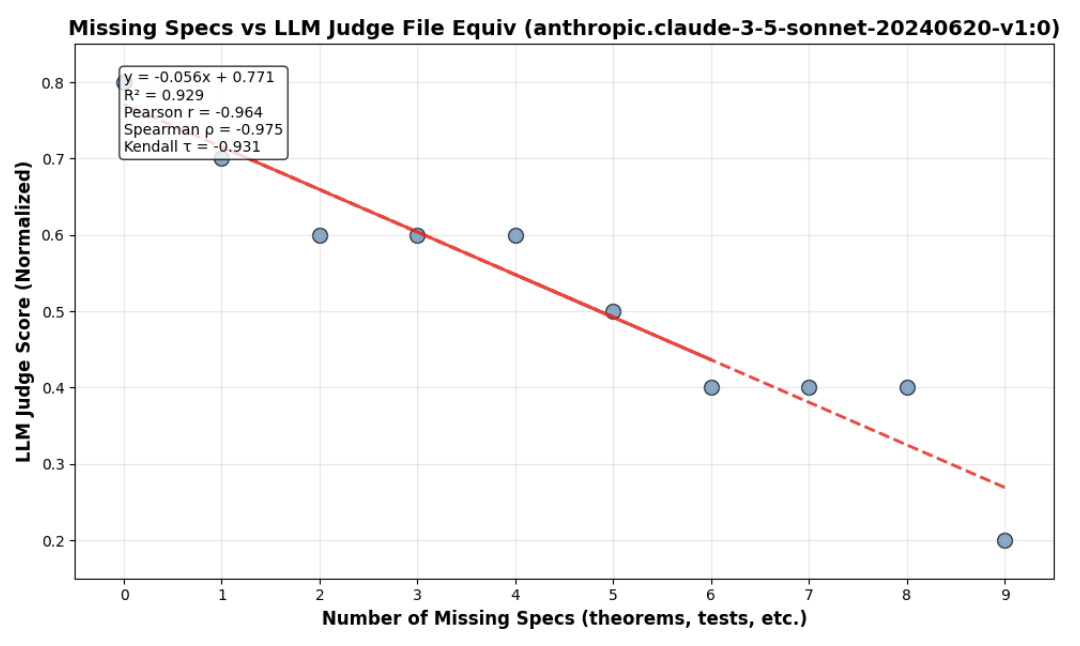
\includegraphics[width=\linewidth]{figures/3.5_specs_missing.png}
    \caption{Monotonicity vs.\ Missing Specs (claude-3-5)}
    \label{fig:app-missing-specs}
  \end{subfigure}\hfill
  \begin{subfigure}[t]{0.48\textwidth}
    \centering
    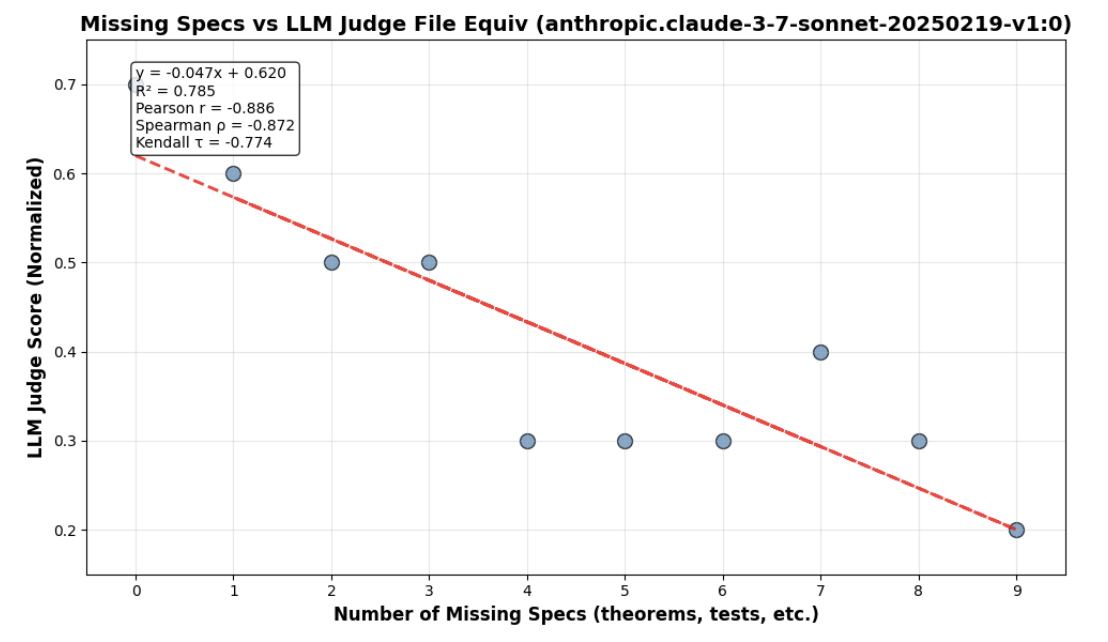
\includegraphics[width=\linewidth]{figures/3.7_specs_missing.png}
    \caption{Monotonicity vs.\ Missing Specs (claude-3-7)}
  \end{subfigure}
  \caption{Missing specs monotonicity across model versions.}
\end{figure}

\begin{figure}[H]
  \centering
  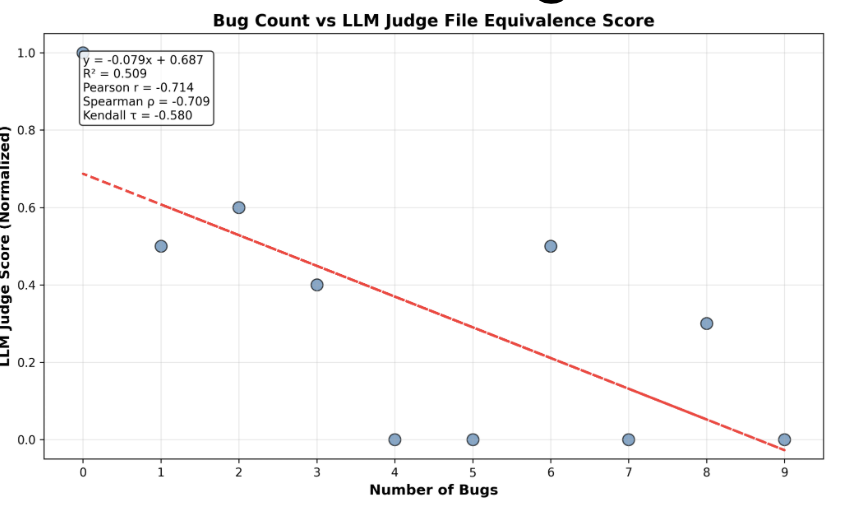
\includegraphics[width=0.5\textwidth]{figures/3.5_bugs.png}
  \caption{Monotonicity vs.\ Bugs (claude-3-5).}\label{fig:app-bugs}
\end{figure}

\end{document}
